\documentclass[a4paper,10pt]{article}
   \usepackage[english]{babel}
   \usepackage{blindtext}
   \usepackage[T1]{fontenc}
   \usepackage{comment}
   \usepackage{graphicx}
   \begin{document}

   \begin{section}{Introduction to mathematics of GemaTreeAC 2=0}
     GemaTreeAC 2=0 is a gematria calculator, numerological classification algorithm and a database.
     Gematria is the mapping of alphabetical characters to numbers by a cipher. The mapping is represented by
     key-value pairs, the key being the letter and value the number. An ordinal cipher would map a to 1, b to 2,
     c to 3 and so on. Words have gematria values, too, according to the cipher. The characters in a word are mapped to
     numbers and their sum is the gematria value of a word. If two words have the same gematria value,
     they are regarded as as semantically related.

     GemaTreeAC has a few more relations than that of the identical gematria value.
     Numerological reduction creates new categories for numbers:
     These are the n-digit set, the root number and the
     route from leaf to root of a number. GeamTreeAC uses this data
     to compete numeral pairs by their numerological properties. The numeral pairs (searched for value and a value
     from the database) gain points when they share a numerological property.
     Gematria value of a word is denoted here by $v$
     
     \[
     \forall v, v \in N_0
     \]


     In parallel with points from numerological properties, the DMS Plot also uses simple distance measures:
     \[d_{property_{v_0,v_1}} = |property_{v_0} - property_{v_1}|\] The distances from
     this process are plotted in a scatter diagram and
     different numerological relations are color coded. In the following formulas, $v_0$
     is the searched for gematria value of a word and $v_1$ is a gematria value of a word found in the database.

     The numerological distance is calculated as
     \[
     \delta_{v_0, v_1} = \frac{  d_{nds_{v_0,v_1}} + d_{root_{v_0,v_1}} + d_{gematria_{v_0,v_1}}  }
     {  points_{nds} + points_{root} + points_{route} + points_{gematria} + points_{word}  }
     \] with some biases and weights to better control the distance measure search results and the plot.

     GemaTreeAC's algorithm uses the distance measure $\delta$ and an angle $\phi$ to calculate the coordinates of a number.
     The angle is expressed as
     \[
     \phi = \frac{v}{v_{max}}*360^\circ \textrm{where $v_{max}$ is the highest $v$ in current search} 
     \]

     In the plot,
     \[
     x = sin\phi*\delta \quad \textrm{and} \quad y = cos\phi*\delta
     \]

     The length of a number means the number of digits in a value, in this context.

     \[
     length_v = \textrm{ number of digits in } v.
     \]

     The n-digit set of $v$ is defined as
     \[
     \nu_v = [10^{length_v-1}, ... , 9*(\sum_{n=0}^{n=length_v-1} 10^n)]
     \]

     It is true that
     \[
     \forall v, v \in \nu_{length_v}
     \]

     Numerological reduction is calculated as
     \[
     parent_v = \sum_{n=0}^{n=length_v-1}v_n
     \]

     The root number is reached when
     \[
     v \in \nu_1
     \]

     The route to root is defined as
     \[
     route_v = [v, f(v)=f(parent_v)]
     \]

     This means that number $666$ has the route $[666, 18, 9]$ and $123$ has the route $[123, 6]$.
     
   \end{section}

   \begin{section}{The DMS Plot}
     The Distance Measure Search and the DMS Plot are the main functions of GemaTreeAC 2=0's database search.
     The result set of the search consists of numerologically related gematria values of words. The DMS parameters
     govern the form of the result set. The only thing that keeps the search having meaningful results is a group
     of 12 parameters that restrict the search. Straight relations to the numbers and their properties are not used.
     Every result set is the consequence of the Distance Measure. The Distance Measure depends on the cipher in use,
     the contents of the database, the searched after word and the DMS parameters. These four factors have to be identical
     to get an identical result set.

     The DMS could be used for cryptography. The receiver has to have the same four factors as the sender. The database in
     GemaTreeAC 2=0 has over 350000 words in Finnish, Swedish and English. The resulting patterns in DMS Plot are unique to
     a word and the contents of the database. The cipher and the parameter set matter, too.

     DMS is also an effective way of mining data. The only problem is that gematria/numerology probably
     does not induce semantics inherently. My experience is that meaning is in the mind of the analyst, not in the numbers.
     Gematria and numerology can be used for divination, prophecies, media analysis, to construct words of power and to
     analyze sacred or otherwise important numbers. Via the kabbalistic symbol of the tree of life, all numbers connect
     to tarot, alchemy, astrology and other occult arts. If numbers had universal meaning, GemaTreeAC should blast truths
     about the Universe constantly, but the secrets it reveals seem more like random.

     I haven't lost hope on the usage of GemaTreeAC in data mining applications, although gematria/numerology does not
     tell Universal truths. The database and the cipher could be formed in such a way, they would produce results that make
     sense. The user of the system would have to define the semantics by an algorithm of some kind or manually. The starting
     point could be synonyms and analogical word pairs. Correspondences of the words would then be used to construct a
     specialized database and a cipher which would yield results that make sense in the chosen context. This application
     of GemaTreeAC could be used for text generation, too. The words could be classified by grammatical properties in a
     way that these properties would align with numerological properties. The starting point could also be syllables and
     their gematria values or then the starting point could be whole sentences. The end result would be a specialized
     cipher and database for use in generation of text in a specific field of information.
     

     \begin{figure}
       \centering
       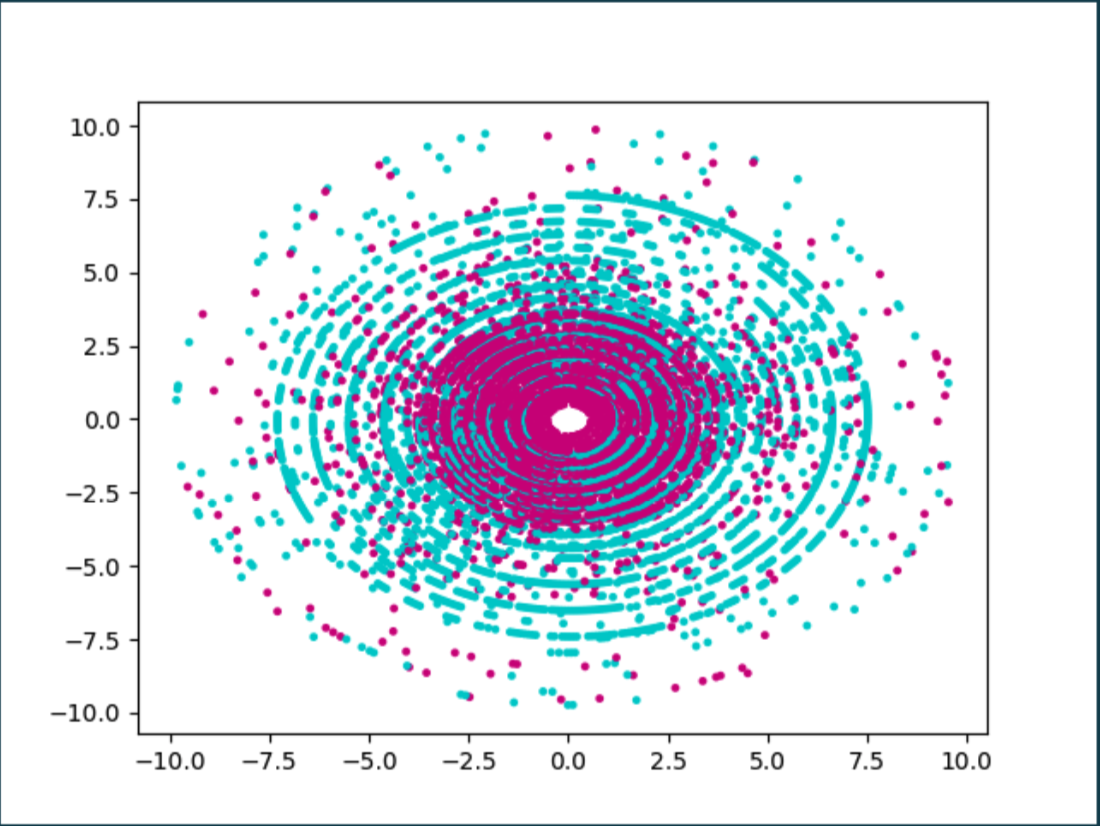
\includegraphics[width = 240px, height = 180px]{suuripetotaivos66360}
       \caption{DMS Plot of word 'suuripetotaivos', gematria 66360 in Fibonacci cipher.}
     \end{figure}

     \begin{figure}
       \centering
       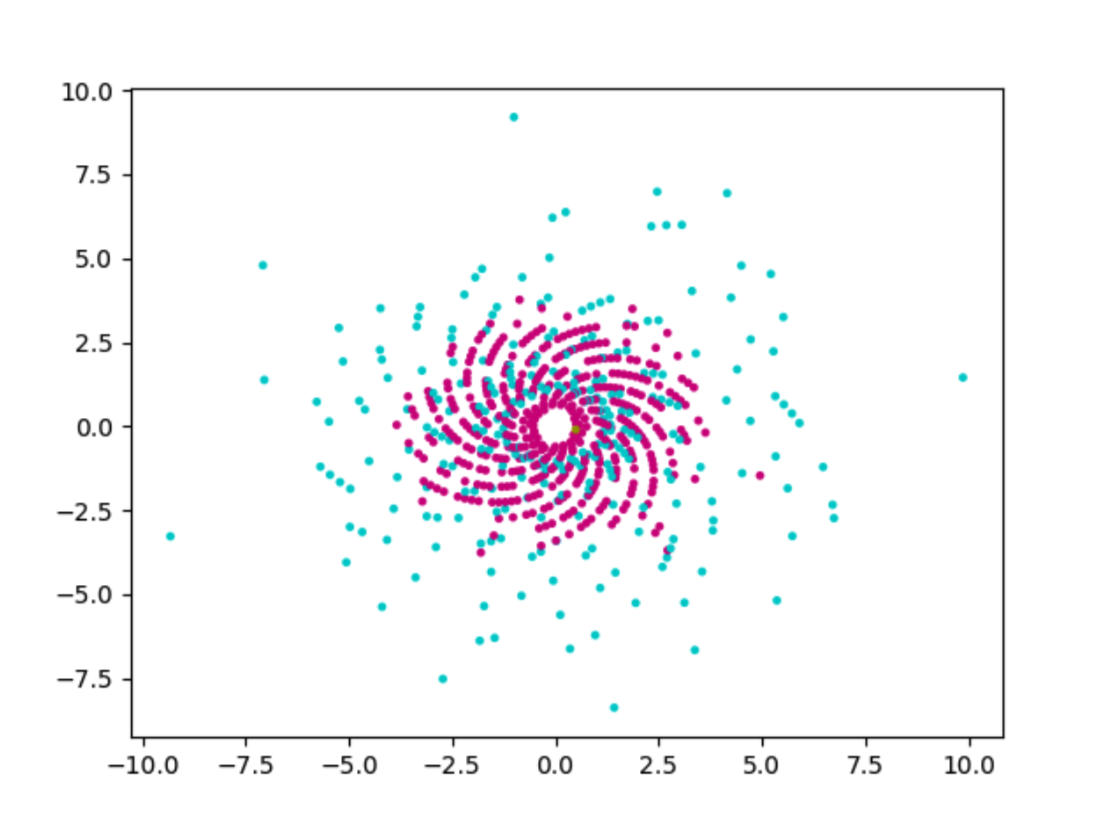
\includegraphics[width = 240px, height = 180px]{komplicerande387}
       \caption{DMS Plot of word 'komplicerande', gematria 387 in English Extended cipher.}
     \end{figure}

     \begin{figure}
       \centering
       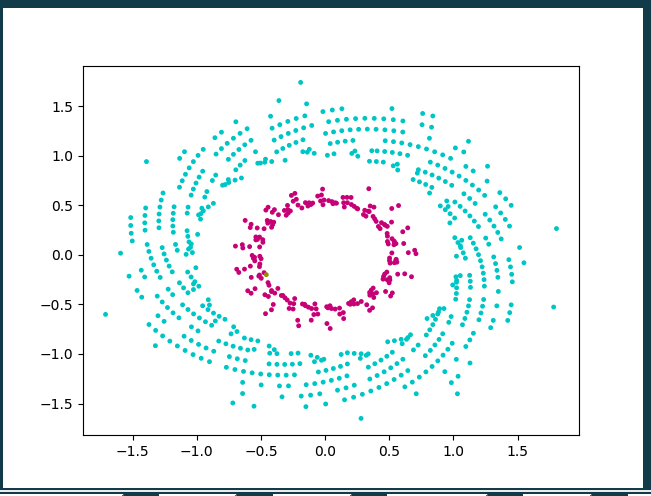
\includegraphics[width = 240px, height = 180px]{suuripeto1134}
       \caption{DMS Plot of word 'suuripeto', gematria 1134 in English Extended cipher.}
     \end{figure}
     
   \end{section}
   

   \end{document}

   
